\subsection{Evaluation Criteria}
The $R^2$ score alone is not sufficient validation in this setting, as accurate ground truth labels are unavailable for data with holes and gaps. Additionally, there exists some unknown uncertainty in the true surface density. To overcome these limitations, we introduce three complementary validation methods to assist the $R^2$ evaluation. All three validation methods are applied to a new, more complex shape called chain-wheel which can be seen on Figure~\ref{fig:chain_wheel}. This shape has not been included in the training dataset, which will provide a good test of the models abillity to generalize to unseen geometries.

\begin{figure}[htbp]
    \centering
    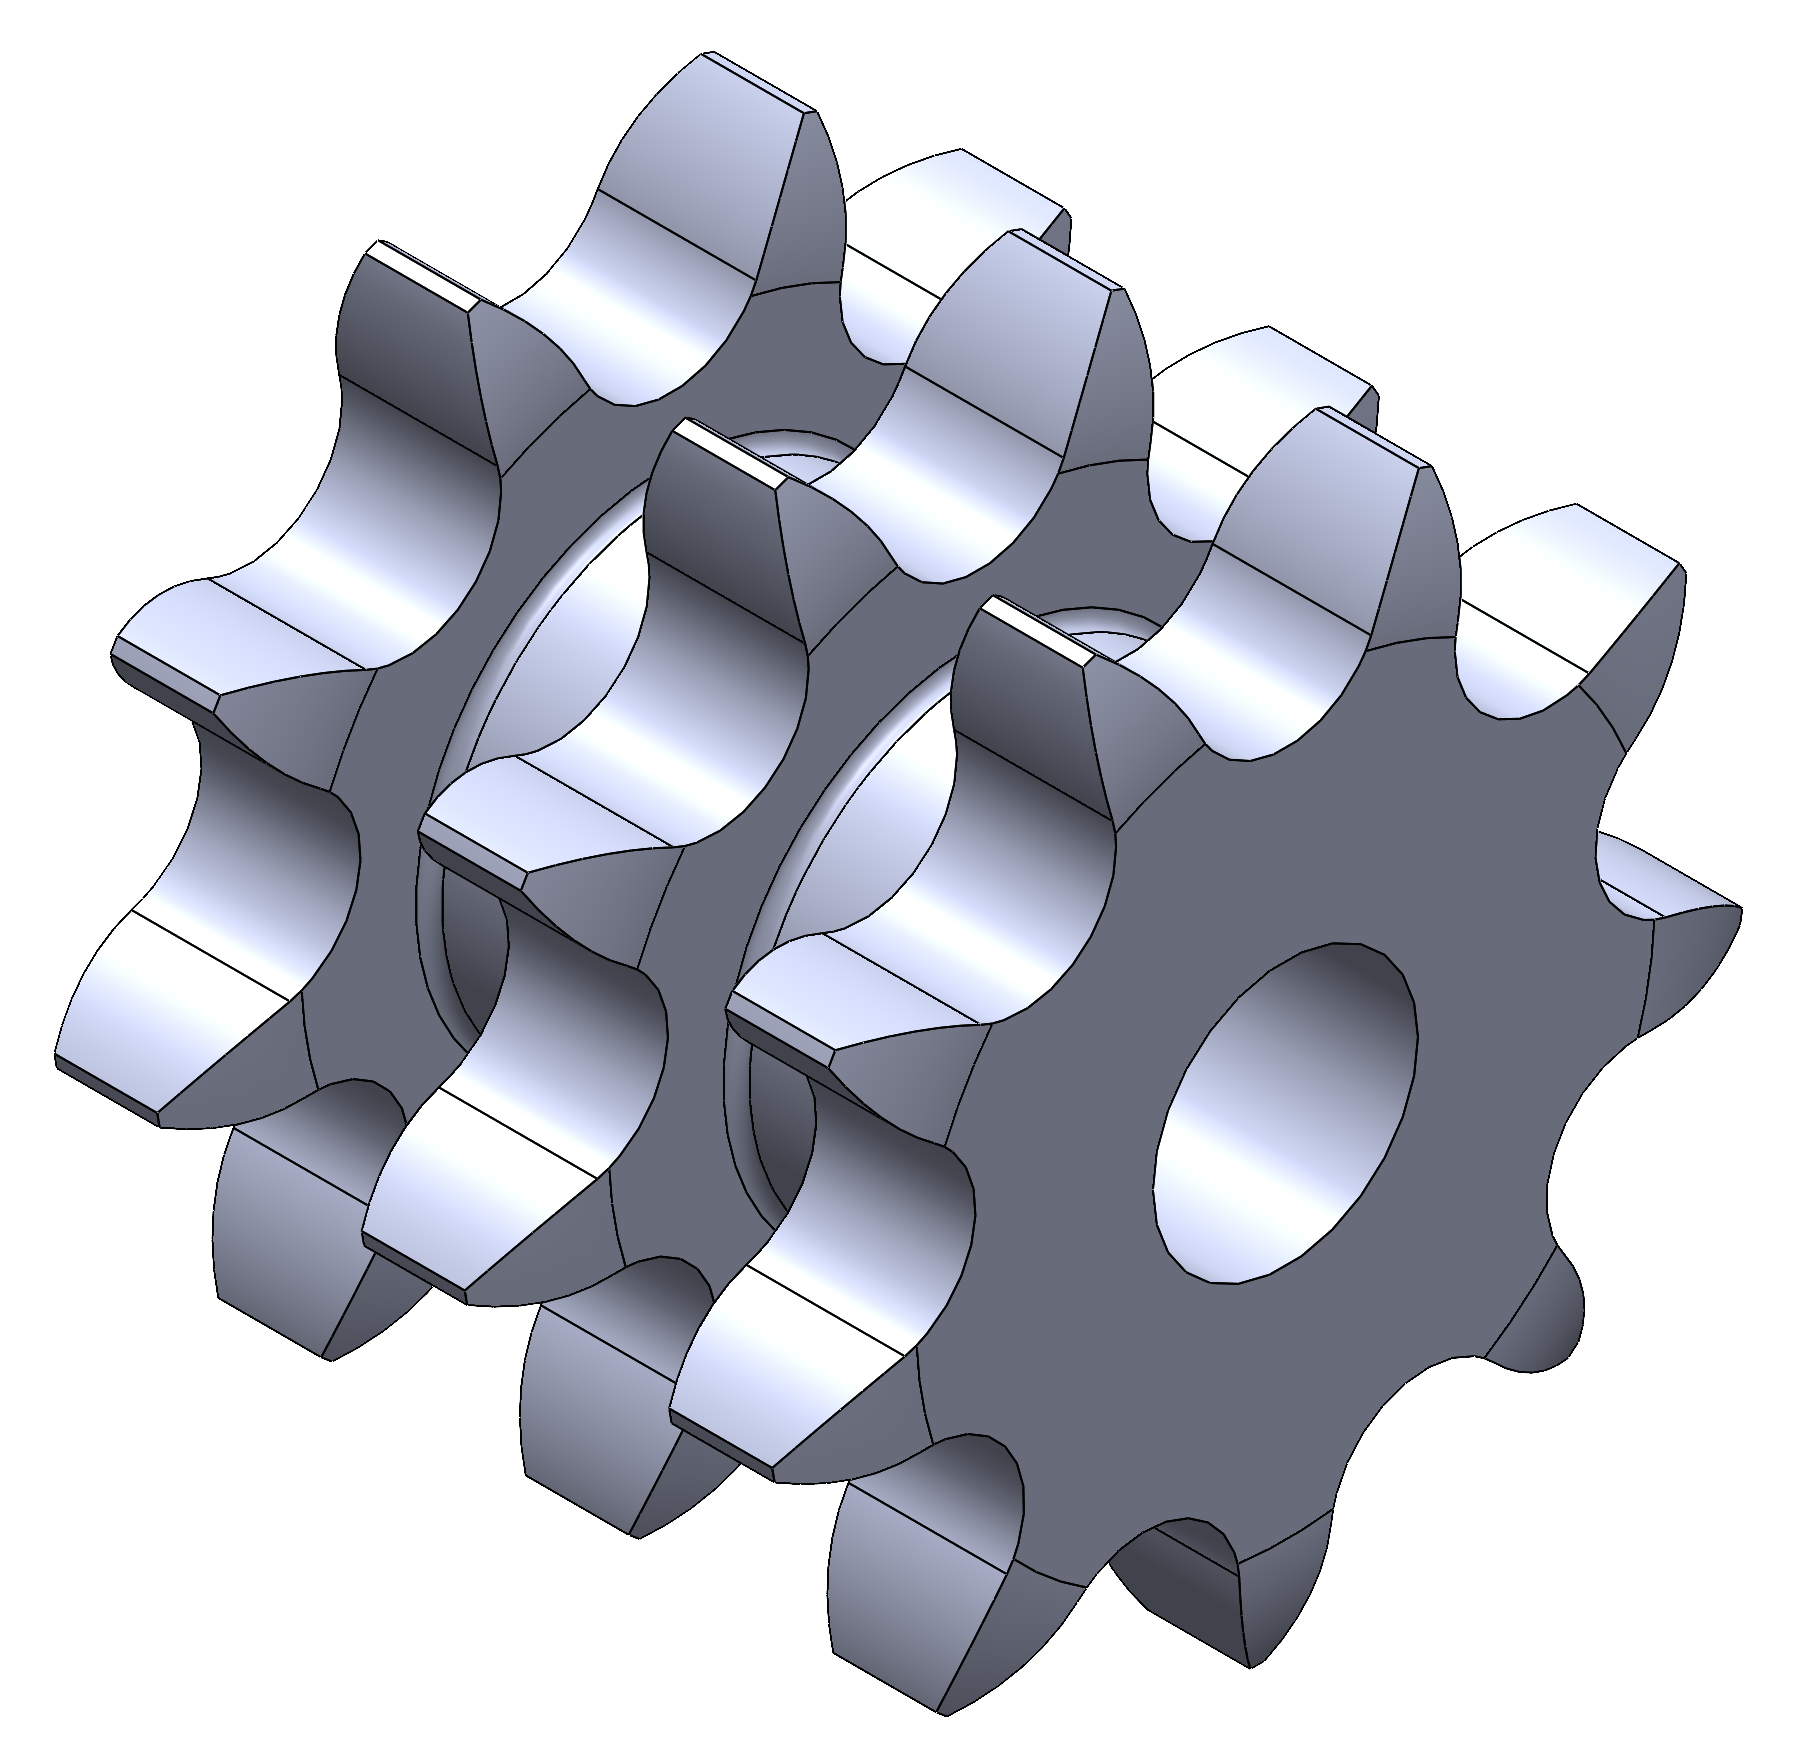
\includegraphics[width=0.3\textwidth]{figures/Chain_whee.PNG}
    \caption{Chain wheel part used for testing the models.} 
    \label{fig:chain_wheel}
\end{figure}

\subsection*{Predict holes}
Testing the models ability to estimate surface density around holes and gaps is challenging due to the lack of reliable ground truth labels. However, the model should at least predict noticeably lower surface density near hole edges. To evaluate this, we generated test datasets with random holes of varying sizes in the point clouds, predictions were then plotted to allow visual identification of hole boundaries in the plots. For smaller holes, a greater number of holes were created to ensure visibility. Six test sets were generated as follows:
\begin{itemize}
    \item \textbf{Holesize: 0, Number of Holes: 0} Control dataset for comparison
    \item \textbf{Holesize: 5, Number of Holes: 60}
    \item \textbf{Holesize: 20, Number of Holes: 50}
    \item \textbf{Holesize: 100, Number of Holes: 30}
    \item \textbf{Holesize: 200, Number of Holes: 20}
    \item \textbf{Holesize: 500, Number of Holes: 10}
\end{itemize}

\subsection*{Estimate label uncertainty}
It is difficult to determine whether the variation and outliers in predicted surface densities are due to model inaccuracies or simply reflect the imperfect ground truth labels. The latter stems from the fact that global surface density is used as a label, even though the meshing tool cannot guarantee uniform surface coverage.
To empirically estimate the uncertainty in the true surface density, we mesh three of the base training shapes (ball, box donut) ten times for each of the meshsizes used during training. Each shape is designed with adaptable dimensions to maintain a surface area corresponding to approximately 160 points at the spcified meshsize. The resulting pointclouds are then devided into eight regions of equal surface area, each containing on average around 20 points. For each region, the local surface density is computed by counting the number of points and deviding by the surface area. This yields 240 surface density samples per mesh size, 80 for each of the three shapes. From these, the empirical mean and standard deviation of the true surface densities can be calculated and directly compared to the distribution of predicted values at each mesh size.

\begin{figure*}[h]
    \centering
    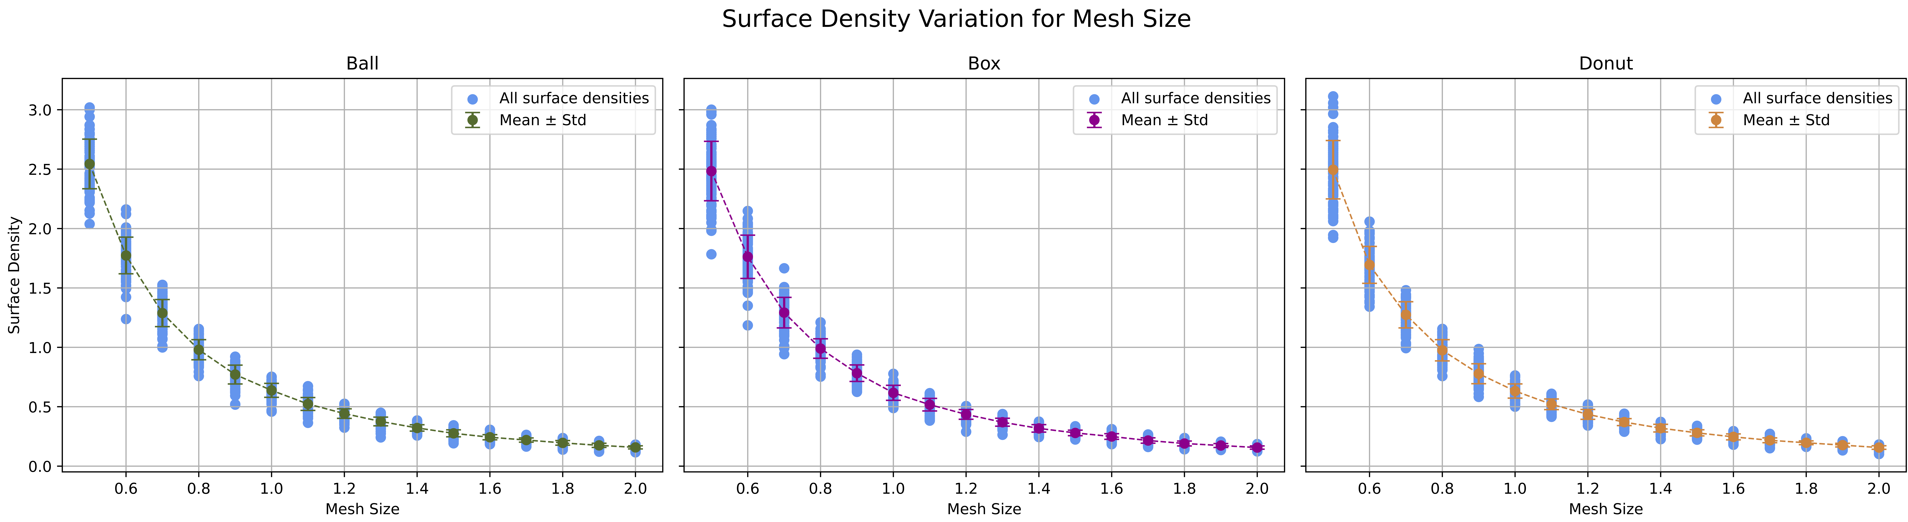
\includegraphics[width=\textwidth]{figures/sd_vs_mesh_lowQ.png}
    \caption{Variation in surface density for different shapes at different mesh sizes}
    \label{fig:sd_mesh}
\end{figure*}

\subsection*{Plot predictions of varying meshsize}
Three point clouds of the same shape are generated using mesh sizes of 0.5, 0.6, and 0.7. Features are computed for each point cloud, and a new composite point cloud with appended features is created by segmenting the geometry into three parts corresponding to the different mesh sizes. This setup evaluates whether the model can predict surface densities with sufficient precision to distinguish between areas of similar mesh size.